\documentclass[12pt,a4paper]{article}

% Margins.
\setlength{\oddsidemargin}{0in}
\setlength{\evensidemargin}{0in}
\setlength{\headheight}{12pt}
\setlength{\headsep}{42pt}
\setlength{\topmargin}{-54pt}
\setlength{\textwidth}{6.5in}
\setlength{\textheight}{10in}

\usepackage{amsmath}
\usepackage{float}
\usepackage{graphicx}
\usepackage[hyphens]{url}
\usepackage{hyperref}	% Clickable links to figures, references and urls.
\usepackage{enumerate}
\usepackage{datetime}

% Drawing.
\usepackage{pgf}
\usepackage{tikz}

% Listings for formatting code.
\usepackage{listings}
\usepackage{textcomp}
% General options.
\lstset{breaklines=true, basicstyle=\small\ttfamily, tabsize=4, numbers=left, stepnumber=1, frame=single, showstringspaces=false, upquote=true}
% C++ specific high-lighting. Comments are 50/50 shades of green/black and strings coloured with 60/40 red/black mixture.
\lstset{language=[ISO]C++, commentstyle=\color{green!50!black}, keywordstyle=\color{blue}, stringstyle=\color{red!60!black}}

%opening
\title{\vspace{-2cm}Programming for Engineers II\\Class 26\\Advanced Pointers\\Keyword \texttt{this}}
\author{Attique Dawood}
\date{July 11, 2013\\[0.2cm] Last Modified: \today, \currenttime}
\begin{document}
\maketitle
\section{Announcements}
\begin{itemize}
\item None.
\end{itemize}
\section{Revision}
\begin{itemize}
\item Dynamic memory allocation using pointer. Object pointers and \verb|->| notation.
\item Pointers and arrays.
\item Pointer levels: double and triple pointers.
\end{itemize}
\section{More on Pointers}
\begin{lstlisting}[caption={Pointer Example},escapechar=!]
#include <iostream>
using namespace std;

int main()
{
	// Note: For the following scenario, p2 was located 12 bytes before p1 in memory.
	// For example, assuming address of p1 was 12, address of p2 would be 0. This can be verified by using debugger.
	int** pp;
	int* p1;
	int* p2;

	int arr1[5] = {6,7,8,9,10};
	int arr2[5] = {1,2,3,4,5};

	p1 = arr1;
	p2 = arr2;
	pp = &p1;

	cout << "&p1: " << &p1 << endl
		 << "p1: " << p1 << endl
		 << "*p1: " << *p1 << endl
		 << "*(p1+0): " << *(p1+0) << endl
		 << "p1[0]: " << p1[0] << endl
		 << "p1[1]: " << p1[1] << endl
		 << "*(p1+2): " << *(p1+2) << endl;

	cout << "&pp: " << &pp << endl
		 << "pp: " << pp << endl
		 << "*pp: " << *pp << endl
		 << "**pp: " << **pp << endl
		 << "*(pp+0): " << *(pp+0) << endl
		 << "pp[0]: " << pp[0] << endl
		 << "*pp[0]: " << *pp[0] << endl
		 << "(*pp)[0]: " << (*pp)[0] << endl
		 << "*(pp[0]): " << *(pp[0]) << endl
		 << "p2: " << p2 << endl
		 << "pp[-3] = *(pp-3): " << pp[-3] << " (Same as p2)" << endl
		 << "*pp[-3]: " << *pp[-3] << endl
		 << "(*pp)[1]: " << (*pp)[1] << endl
		 << "*(pp[-3]): " << *(pp[-3]) << endl;

	return 0;
}
\end{lstlisting}
\begin{figure}[H]
\centering
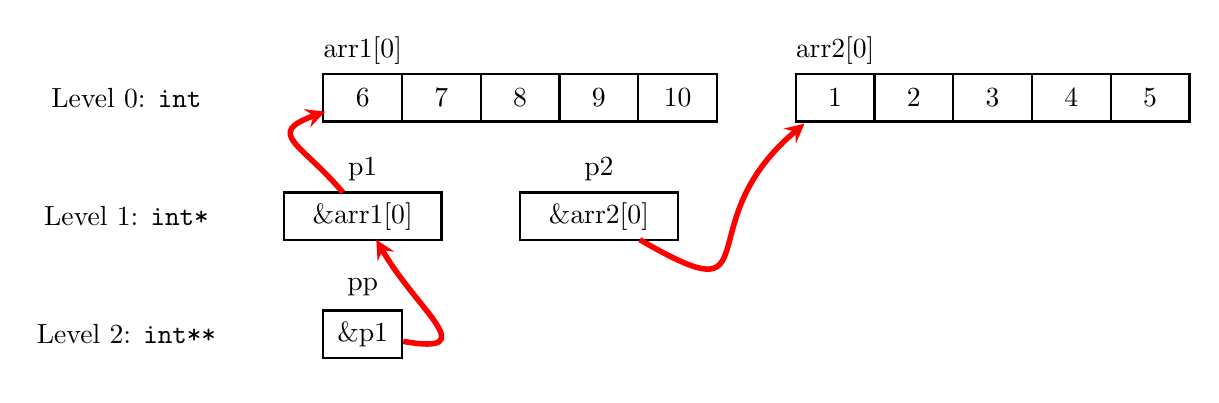
\begin{tikzpicture}
	% int
	\def\yd{0cm}
	\draw (0cm,\yd) node {Level 0: \texttt{int}};
	\foreach \x/\t/\val in {3cm/6/arr1[0], 4cm/7/, 5cm/8/, 6cm/9/, 7cm/10/, 9cm/1/arr2[0], 10cm/2/, 11cm/3/, 12cm/4/, 13cm/5/}
	{
		\draw[thick] (\x-0.5cm, \yd+0.3cm) rectangle (\x+0.5cm, \yd-0.3cm);
		\node[circle,minimum size=1cm] (\val) at (\x,\yd) {\t};
		\draw (\x,\yd+0.6cm) node {\val};
	}
	% int*
	\def\yd{-1.5cm}
	\draw (0cm,\yd) node {Level 1: \texttt{int*}};
	\foreach \x/\t/\val in {3cm/\&arr1[0]/p1, 6cm/\&arr2[0]/p2}
	{
		\draw[thick] (\x-1cm, \yd+0.3cm) rectangle (\x+1cm, \yd-0.3cm);
		\node[] (\val) at (\x,\yd) {\t};
		\draw (\x,\yd+0.6cm) node {\val};
	}
	\draw[thick,red,>=stealth,->,line width=2pt] (p1) to [looseness=2,out=130,in=200] (arr1[0]);
	\draw[thick,red,>=stealth,->,line width=2pt] (p2) to [looseness=2,out=-30,in=220] (arr2[0]);
	% int**
	\def\yd{-3cm}
	\draw (0cm,\yd) node {Level 2: \texttt{int**}};
	\foreach \x/\t/\val in {3cm/\&p1/pp}
	{
		\draw[thick] (\x-0.5cm, \yd+0.3cm) rectangle (\x+0.5cm, \yd-0.3cm);
		\node[circle,minimum size=1cm] (\val) at (\x,\yd) {\t};
		\draw (\x,\yd+0.6cm) node {\val};
	}
	\draw[thick,red,>=stealth,->,line width=2pt] (pp) to [looseness=2,out=-10,in=-60] (p1);
\end{tikzpicture}
\caption{Accessing array using pointer}
\label{Accessing-Array-as-Pointer}
\end{figure}
\section{\texttt{this} Pointer}
\begin{itemize}
\item Inside class functions, we have access to a `magic' pointer named \verb|this|.
\item This pointer points to calling object itself.
\end{itemize}
\begin{lstlisting}[caption={\texttt{this} pointer}]
#include <iostream>
using namespace std;

class Complex
{
	private:
	float real;
	float img;
	public:
	Complex()
	{
		cout << "My object's address is: " << this << endl;
	}
	void Input()
	{
		cin >> this->real;
		cin >> this->img;
	}
	void Display()
	{
		cout << this->real << endl;
		cout << this->img << endl;
	}
};

int main()
{
	Complex c;
	c.Input();
	c.Display();

	return 0;
}
\end{lstlisting}
\section{Returning By Reference Using \texttt{this}}
\begin{lstlisting}[caption={Returning by reference using \texttt{this} pointer},escapechar=!]
class Complex
{
	private:
	float real;
	float img;
	public:
	Complex& operator= (Complex & rhs)
	{
		real = rhs.real;
		img = rhs.img;
		return (*this);
	}
};
int main()
{
	Complex A, B, C;
	!\color{red}{A = B = C}!;

	return 0;
}
\end{lstlisting}
\section{\texttt{sizeof() struct or class}}
\begin{itemize}
\item If there is only one data member then size of object is the size of data member. For example size of \verb|class X { char t; }| object is 1 byte.
\item For default settings, if there are more than 1 members then size is a multiple of `struct package size'. Default package size is 8 bytes.
\item A class with one char and one double is 9 bytes, so with default package size object will be of 16 bytes in memory.
\end{itemize}
\begin{figure}[H]
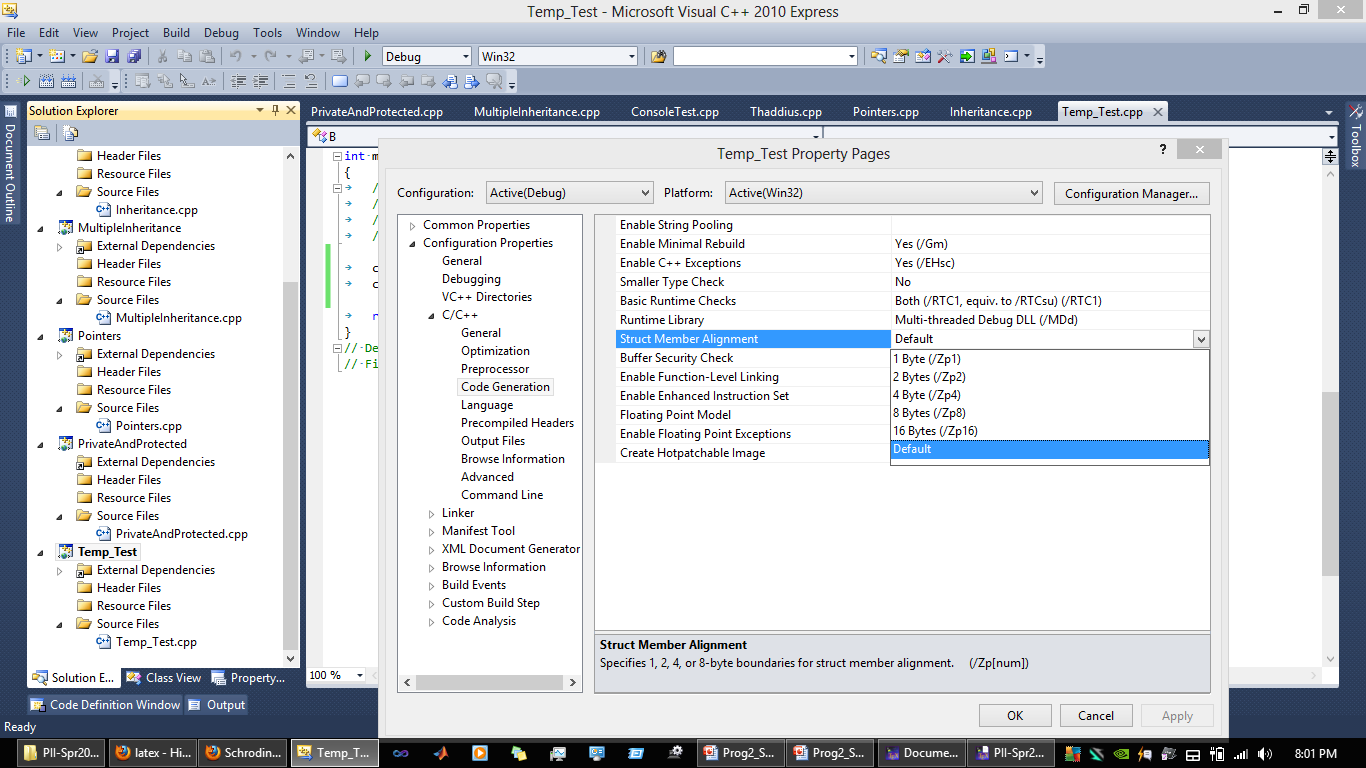
\includegraphics[width=\textwidth]{StructPackagingSize}
\end{figure}
\section{\texttt{void} Pointers}
\begin{itemize}
\item What if you don't know the type of data you're going to dynamically allocate?
\item Solution: Make a \verb|void*|. It can point to any datatype!
\item \underline{Must explicitly cast the pointer when accessing value.}
\end{itemize}
\begin{lstlisting}[caption={\texttt{void*} usage}]
#include <iostream>
using namespace std;

int main()
{
	void* vp;
	vp = new int[5];
	delete[] vp;

	vp = new float;
	*((float*)vp) = 3.3f; // Notice, explicit casting from void* to float* before dereferencing.
	cout << "*vp: " << *((float*)vp) << endl;
	delete vp;

	return 0;
}
\end{lstlisting}
\section{\texttt{const} Pointers}
\begin{lstlisting}[caption={\texttt{const} pointers}, escapechar=!]
!\color{red}{const int*}! p; // Value pointed by pointer is constant.
int* !\color{red}{const p}!; // Pointer is constant. Can only point to one thing.
\end{lstlisting}
\section{Constant String}
\begin{lstlisting}[caption={constant string}]
#include <iostream>
using namespace std;

int main()
{
	char str1[] = "Defined as an array";
	char* str2 = "Defined as a pointer";
	cout << str1 << endl; // display both strings
	cout << str2 << endl;
	//str1++; //can’t do this; str1 is a const ptr
	str2++; // this is OK, str2 is a pointer
	cout << str2 << endl; //now str2 starts "efined..."

	return 0;
}
\end{lstlisting}
\begin{lstlisting}[caption={Array of constant strings, contiguous storage}]
#include <iostream>
using namespace std;

int main()
{
	const int DAYS = 7;
	char* arrptrs[DAYS] = { "Sunday", "Monday", "Tuesday", "Wednesday", "Thursday", "Friday", "Saturday" };

	for(int j=0; j<DAYS; j++) //cout every string
		cout << arrptrs[j] << endl;

	return 0;
}
\end{lstlisting}
\begin{lstlisting}[caption={Constant column length, non-contiguous storage},escapechar=!]
#include <iostream>
using namespace std;

int main()
{
	const int DAYS = 7;
	!\color{red}{char arrptrs[DAYS][10]}! = { "Sunday", "Monday", "Tuesday", "Wednesday", "Thursday", "Friday", "Saturday" };

	for(int j=0; j<DAYS; j++) //cout every string
		cout << arrptrs[j] << endl;

	return 0;
}
\end{lstlisting}
%\nocite{*}
%\bibliographystyle{plain}
%\bibliography{OOPref}
\end{document}
